%!TEX root=ZR_bmicha_SysMod.tex

\subsection{Hydraulic Duct}
    \begin{minipage}{0.67\linewidth}
        \begin{center}
            \resizebox{\linewidth}{!}{
            \includegraphics[
                    page = {36},
                    trim = {6.5cm, 11cm, 6.5cm, 11.5cm}, %l b r t
                    clip
                ]{External/Skript.pdf}
            }
        \end{center}
    \end{minipage}
    \begin{minipage}{0.31\linewidth}
        \begin{center}
            \resizebox{\linewidth}{!}{
            
\includegraphics[
                    page = {5},
                    trim = {17cm, 1cm, 9cm, 11.25cm}, %l b r t
                    clip
                ]{Hydraulic-Systems/SlidesEx02.pdf}
            }
        \end{center}       
    \end{minipage}
    \textbf{Newton's Law} yields:
    \mathbox{
        \frac{d}{dt}v(t) = \frac{1}{\rho l} (p_1(t) - p_2(t)) + \frac{g h}{l} - \frac{F_{fric}(t)}{\rho l A}
    }
    $$
        F_{fric}(t) = A \cdot \lambda(v(t)) \cdot \frac{l}{d} \cdot \frac{\rho}{2} \cdot v^2(t) \cdot sgn(v(t))
    $$
\subsection{Compressible Duct}
    \begin{minipage}{0.68\linewidth}
        \begin{center}
            \resizebox{\linewidth}{!}{
            \includegraphics[
                    page = {37},
                    trim = {7cm, 13cm, 7cm, 12cm}, %l b r t
                    clip
                ]{External/Skript.pdf}
            }
        \end{center}
    \end{minipage}
    \begin{minipage}{0.31\linewidth}
        \begin{center}
            \resizebox{\linewidth}{!}{
            
\includegraphics[
                    page = {8},
                    trim = {17cm, 1cm, 9cm, 11.5cm}, %l b r t
                    clip
                ]{Hydraulic-Systems/SlidesEx02.pdf}
            }
        \end{center}       
    \end{minipage}
    
    \mathbox{
        \frac{d}{dt}V(t) = \dot{V}_{in} - \dot{V}_{out} = A_{in} \cdot v_{in} - A_{out} \cdot v_{out}
    }
    \mathbox{
        p(t) = \frac{1}{\sigma_0} \cdot \frac{V(t) - V_0}{V_0} + p_{static}
    }
    $$
        \sigma_0 = \frac{1}{V_0} \cdot \frac{dV}{dp} \qquad \left[\frac{1}{Pa}\right]
    $$
\subsection{Valve}
    \vspace{-1em}
    \begin{center}
        \resizebox{\linewidth}{!}{
            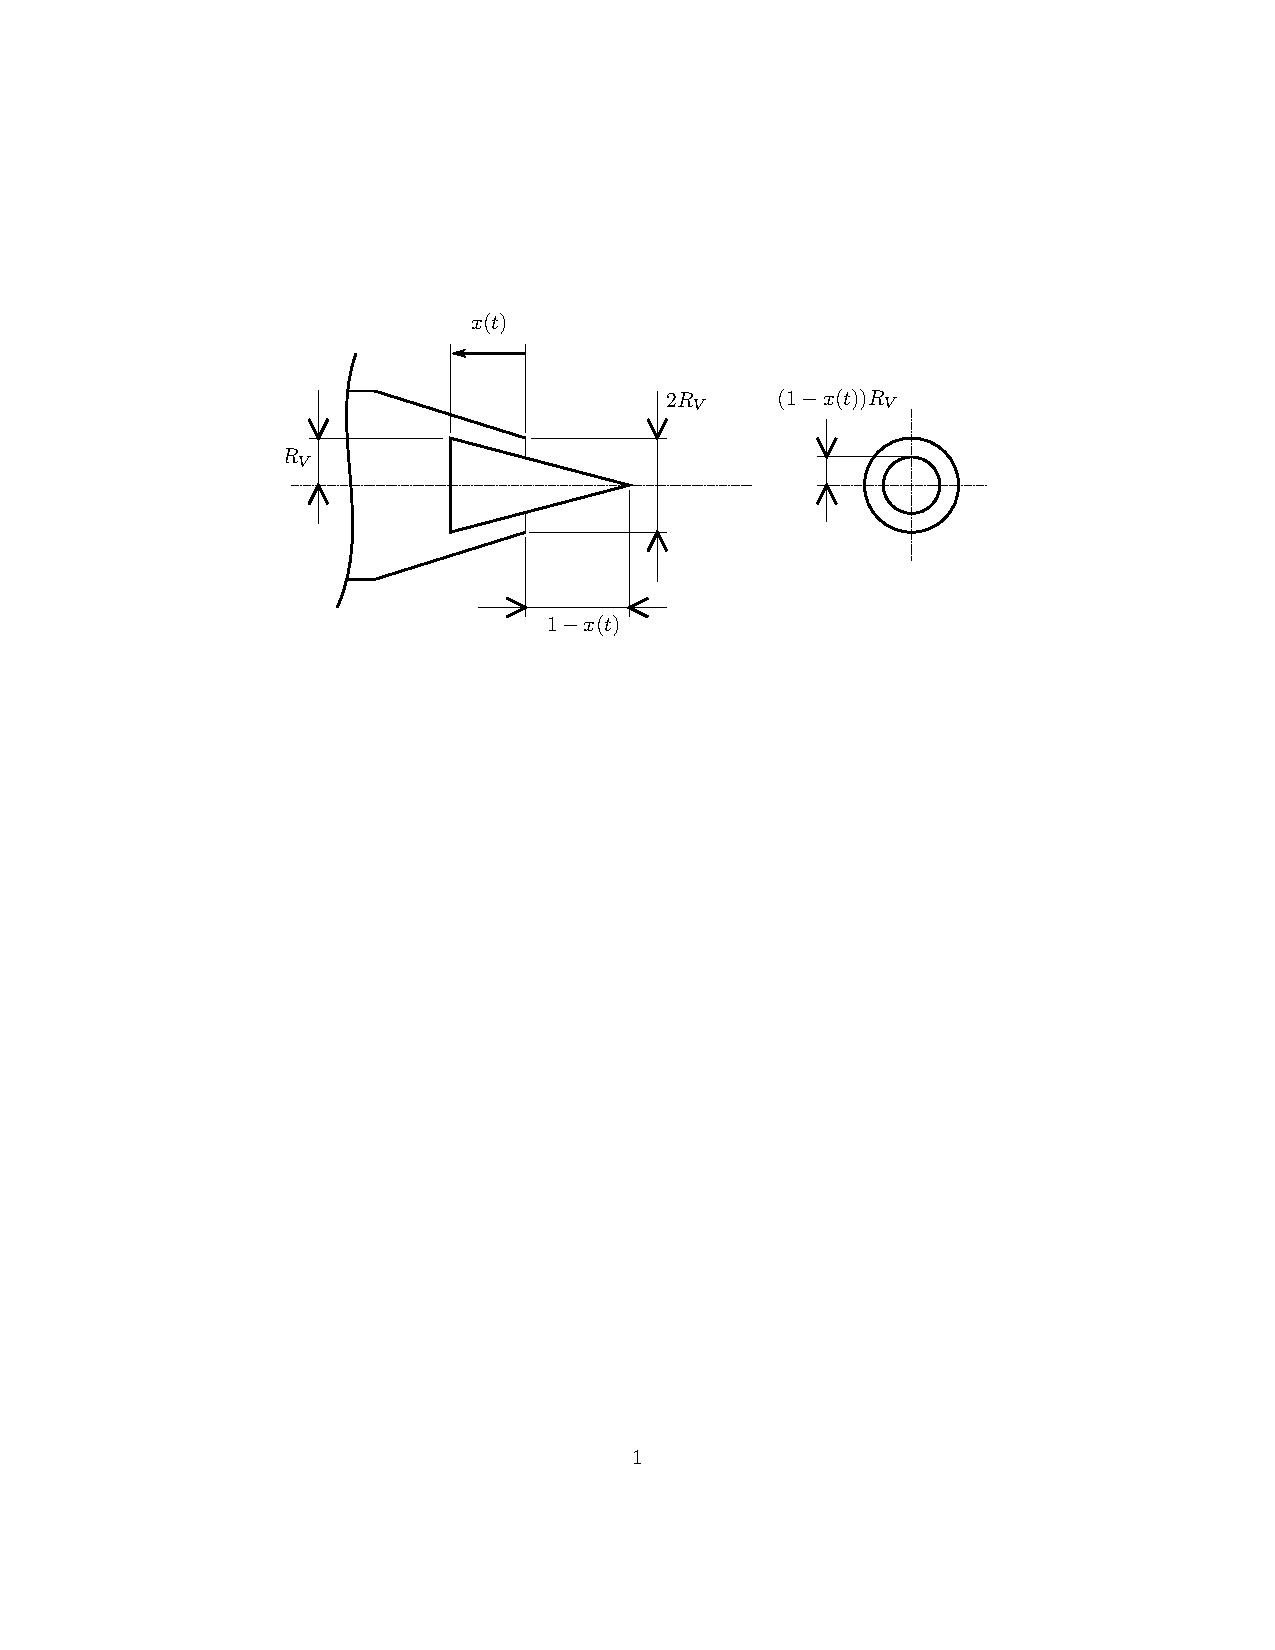
\includegraphics[
                page = {1},
                trim = {4cm, 17cm, 5cm, 5cm}, %l b r t
                clip
            ]{Hydraulic-Systems/valve.pdf}
        }
    \end{center}
    \textbf{Opening Area of the Valve:}
    \begin{align*}
        A_V(t) &= \pi \cdot R_V^2 - \pi \cdot \left( (1-x(t)) \cdot R_V\right)^2\\
        &= A_{V0} \cdot \left( 1 - (1-x(t))^2 \right)
    \end{align*}
    \textbf{Flow Velocity of \textit{Incompressible} Medium}
    $$
        v_V(t) = c_d \cdot \sqrt{\frac{2 \cdot (p_F(t) - p_0)}{\rho}}, \qquad v_V \gg v_{in}
    $$
        